\section{Crypto Recap}
\subsection{Objectives:}
\begin{itemize}
  \item{\textbf{Confidentiality}}
  \item{\textbf{Integrity}}
  \item{\textbf{Authenticity}}
  \item{\textbf{Availability}}
  \item{Authorization}
  \item{Non-Repudiation, Accountability}
  \item{Freshness}
  \item{Anonymity, Unlinkability}
  \item{Intervenability, Contro}
  \item{Transparency}
\end{itemize}

\subsection{Confidentiality-Encryption}
\subsubsection{Symmetric Ciphers}
\begin{itemize}
  \item Secret key for en- and decryption
  \item Much more efficient
  \item \textbf{Block cipher: }encryps a plaintext block of fixed len e.g.: \textit{Advanced Encryption Standard (AES)}
  \item \textbf{Stream cipher: }encrypts a bitstream e.g.:\textit{ChaCha20}
\end{itemize}

\subsubsection{Asymmetric Ciphers}
\begin{itemize}
  \item Public key for encryption
  \item Private key for decryption
  \item Ex.: RSA-based encryption
\end{itemize}

\subsection{Integrity, Authenticity-Signatures, MACs}
\subsubsection{MACs}
\begin{itemize}
  \item Symmetric cryptography
  \item Protects data integrity \& authenticity
  \item Ex.: Hash-based MAC
\end{itemize}

\subsubsection{Digital Signatures}
\begin{itemize}
  \item Asymmetric cryptography
    \begin{itemize}
      \item{\textbf{Signing with} private key}
    \end{itemize}
  \item{Protects data integrity \& authenticity}
  \item{Provices non-repudation}
\end{itemize}

\subsection{Block Cipher Modes of Operation}
\subsubsection{Electronic Code Book (ECB)}
\begin{itemize}
  \item{Each plaintext block is encrypted seperatly}
  \item{Inherintly insecure! -> Smae block = Same cipher}
\end{itemize}

\subsubsection{Cipher Block Chainning (CBC)}
\begin{itemize}
  \item Plaintext is chained to previous ciphertext by XOR and encrypted afterwards
  \item Difficult to apply securely -> implementations often vulnerable
\end{itemize}

\subsubsection{Galois Counter Mode (GCM)}
\begin{center}
  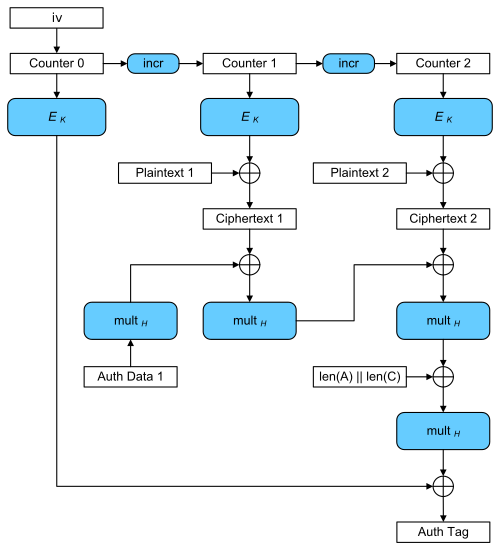
\includegraphics[width=0.5\columnwidth]{Resources/GCM-Galois_Counter_Mode_with_IV.svg.png}
\end{center}

\section{Tranport Layer Security (TLS)}
\subsection{TLS handshake protocol}
\begin{itemize}
  \item Parameter Negotiation
  \item Key exchange
  \item Authentication
\end{itemize}
\subsection{TLS record protocol}
\begin{itemize}
  \item Protection of integrity, authenticiy and confidentiality
  \item \textbf{Symmetric Cryptography:} e.g., block cipher, usually AES
\end{itemize}


\section{Wireless Security}
\subsection{WiFi Security}
\subsubsection{Historic Overview}
\begin{itemize}
  \item 1999: WEP (Wired Equivilaent Privacy)
    \begin{itemize}
      \item Goal: "as secure as a wired LAN"
      \item Insecure, various attacks known
    \end{itemize}
  \item 2003: WPA (WiFi Protected Access)
    \begin{itemize}
      \item Improved protocols; most known attacks on WEP prevented
      \item Enterprice Mode
      \item But: Requirement ofr hardware-compatibility with WEP devices => Encryption improved, but still based on obsolete stream cipher
    \end{itemize}
  \item 2004: WPA2 (still used) 
    \begin{itemize}
      \item Similar to WPA, but AES-based encryption: AES-CCMP
    \end{itemize}
  \item 2018: WPA3 (supported by new devices) 
    \begin{itemize}
      \item Serveral improvements: 
        Prevention of offline-attacks on pre-shared keys, forward secrecy, encryption for "open" WLANs
    \end{itemize}
\end{itemize}
\subsubsection{WPA/WPA2 Security}
\begin{itemize}
  \item Personal Mode
    \begin{itemize}
      \item Pre-Shared Keys
    \end{itemize}
  \item Enterprise Mode 
    \begin{itemize}
      \item EAP-TLS, PEAP, EAP-TTLS
    \end{itemize}

\textbf{AES-CCMP}\\
  \item Authenticated Encryption with Associated Data (AED)
  \item AES-CCM
    \begin{itemize}
      \item Authentication: CBC-MAC
      \item Encryption: Counter Mode (CTR)
      \item MAC and encyprion: computed simultaneously
    \end{itemize}
\end{itemize}

\textbf{4-Way Handshake}\\
\begin{itemize}
  \item Based on Pairwise Master Key (PMK)
    \begin{itemize}
      \item Personal Mode (WPA-PSK):
        Computed from passphrase and SSID (as "salt") using PBKDF2 (password-based key derivation function)
      \item Enterprise Mode: Established by key exchange protocol (e.g. EAP-TLS, PEAP)
    \end{itemize}
  \item 4-Way HS to derive Pairwise Transient Key (PTK) 
    \begin{itemize}
      \item Exchance nonces
      \item PTK is derived by hashing PMK, nonces, MAC addrs 
      \item Furhter key (for differnet purposes) derived from PTK 
      \item Client gets Group Temporary Key from AP (encrypted) 
      \item Message Integrity Code(MIC): MACs for integrity protection, key confirmation 
    \end{itemize}
  \item KRACK (2018): Key reinstallation attacks => meanwhile prevented by software/firmware updates 
  \item Problem: Offline attacks against passphrase 
\end{itemize}

\subsubsection{WPA 3 Improvements}
\begin{itemize}
  \item Mandatory Protected Managment Frames
    \begin{itemize}
      \item Prevents deauthentication attacks (DoS)
    \end{itemize}
  \item Replace PSK Authentication with SAW protocol 
    \begin{itemize}
      \item Simultaneous Authentication among Equals (SAE):
        "Dragonfly" handshake
      \item Prevents offline attacks on passphrase 
      \item Based on elliptic curve cryptography by default
    \end{itemize}
  \item Forward Secrecy based on Diffie-Hellman 
  \item 192-bit Security Mode (optional) 
    \begin{itemize}
      \item AES-256 (GCM)
      \item SHA-384 
      \item 284-bit elliptic curves or RSA with at least 3K bits 
    \end{itemize}
\end{itemize}

\subsubsection{Simultaneous Authentication among Equals}
\begin{itemize}
  \item SAE "Dragonfly" authenicates participants and establishes PMK
    \begin{itemize}
      \item Based on passphrase and (EC-)Diffie-Hellman
      \item Can be initiated simultaneously by both parties (useful for mesh networking) 
    \end{itemize}
  \item 4-Way Handshake 
    \begin{itemize}
      \item Esablishes PTK basen on PMK
      \item Same as in WPA2 
      \item But now: PMK with much higher entropy => Offlione attacks not practical 
    \end{itemize}
  \item Hash-to-Group: "Hunting and Pecking" 
    \begin{itemize}
      \item Generate point on elliptic curve from pasphrase (and MAC addresses, etc.)
      \item Cryptographic has function generates pseudo random numbers (by including a counter in the input) 
        \begin{itemize}
          \item Both parties must use the exact same inputs in the same order
        \end{itemize}
      \item Fixed procedure to derive x-coordinate 
        \begin{itemize}
          \item Check if point on curve can be generated
          \item If check fails: increase coutner and try again 
        \end{itemize}
    \end{itemize}
  \item Auth-Commit messages
    \begin{itemize}
      \item Exchange ECDH shares
    \end{itemize}
  \item Auth-Confirm messages 
    \begin{itemize}
      \item Key confirmation, authentication of messages
    \end{itemize}
\end{itemize}

\subsection{Bluetooth Security}
\begin{itemize}
  \item Authentication: device authentication, no user authentication
  \item Pairing/bondig: create shared keys; used in connections later on 
  \item Confidentiality: encryption of BT communication 
  \item Message Integrity: MACs (authenticated encryption) to protect BT communication 
  \item Authorization: control access to resources (based on devices, not users) 
  \item Security Modes 
    \begin{itemize}
      \item Mode 1: no security
      \item Mode 2: service level (only for backward compatibility) 
      \item Mode 3: link-level enforces security (only for backward compatibility) 
      \item Mode 4: authenticated link key using "Secure Connections", based on device pairing 
    \end{itemize}
  \item Eavesdropptin not trivial: Bluetooth uses frequency hoppting (not a security feature) 
\end{itemize}

\subsubsection{Device Pairing}
\begin{itemize}
  \item Authentication and generation of link key / long term key
  \item PIN/Legacy Pairing: enter PIN on both devices 
    \begin{itemize}
      \item Key generation based on PIN, device address, and random values
    \end{itemize}
  \item Secure Simple Pairing (SSP): since Bluetooth 2.1 
    \begin{itemize}
      \item Numeric Comparison
        \begin{itemize}
          \item Compare 6-digit numbers
        \end{itemize}
      \item Passkey Entry 
        \begin{itemize}
          \item Read 6-digit form one device, enter on the other one
        \end{itemize}
      \item Just Works 
        \begin{itemize}
          \item User accepts connection without verification
        \end{itemize}
      \item Out of Band (OOB) 
        \begin{itemize}
          \item Transmit data using other communication channels (e.g. NFC)
        \end{itemize}
    \end{itemize}
\end{itemize}

\subsubsection{Simple Secure Pairing (SSP)}
\begin{itemize}
  \item Unauthenticated ECDH
  \item 2-Stage Authentication 
    \begin{itemize}
      \item Stage 2: depends on pariing method
      \item Stage 2: Cryptographic authentication based on Stage 1 values and ECDH secret 
    \end{itemize}
  \item Key derivation to generate link key / long term key 
\end{itemize}

\subsubsection{Secure Authentication}
\begin{itemize}
  \item Paired (bonded) devices authenticate each other
  \item Challange-Response scheme 
    \begin{itemize}
      \item 128-bit random challanges
      \item Response: HMAC of BT addresses and challanges (using link key from pairing) 
        \begin{itemize}
          \item Before Bluetooth 4.1: based on Bluetooth-specific algorithm E1
        \end{itemize}
    \end{itemize}
  \item Authenication failure: introcude delay (exponential back-off) 
\end{itemize}

\subsubsection{Confidentiality}
\begin{itemize}
  \item Bluetooth-specific stream cipher E0
    \begin{itemize}
      \item Designed for efficiency
      \item Serious attacks hve been published 
      \item "Practical" in theory (but complex, hard to apply in practice) 
    \end{itemize}
  \item AES-CCM 
    \begin{itemize}
      \item Used since Bluetooth 4.1
      \item Key derived from link key (pairing) and the authentication step 
    \end{itemize}
\end{itemize}

\subsubsection{Privacy}
\begin{itemize}
  \item Privacy problem: Devices (users) can be identified by Bluetooth MAC addresses
  \item Mitigation: BLE private device addresses 
    \begin{itemize}
      \item Resolvable Private Address (RPA) is changed periodically
      \item Identity Address remains constant (but is not transmitted over the air) 
      \item Identity Resolving Key to map RPA to Identity Address 
      \item Especially imprtant to discoverable devices (which advertice identity info) 
    \end{itemize}
\end{itemize}

\subsubsection{5.x Security}
\begin{itemize}
  \item No major changes to security protocols and algorithms
  \item Bluetooth 5.0 
    \begin{itemize}
      \item PHY improvements, no relevant security changes
    \end{itemize}
  \item Bluetooth 5.1 
    \begin{itemize}
      \item HCI support for debug keys (should not be relevant in production systems)
    \end{itemize}
  \item Bluetooth 5.2: adds new features (Extended Attributes, Isochronous Communication, ...)
    \begin{itemize}
      \item Isochronous communication: connection-oriented or connection-less
        \begin{itemize}
          \item Group communication: group keys need to be established
          \item Broadcast Authenication 
        \end{itemize}
    \end{itemize}
  \item Bluetooth 5.3: Key Size Negotiation 
    \begin{itemize}
      \item Enables host to define minimun key size
    \end{itemize}
\end{itemize}

\subsubsection{BLUFFS}
\begin{itemize}
  \item BLUFFS: New attacks against bluetooth
    \begin{itemize}
      \item Breaks Forward Secrecy and Future Secrecy
      \item Enables man-in-the-middle attacks, impersonation if one session key compromised 
      \item Forces weak key: spec allows minimus of 7 Bytes entropy (56 Bits) 
        \begin{itemize}
          \item Brute-force attack: offline, parallelizable
          \item Forces reuse of compromised key 
        \end{itemize}
      \item Attack against bluetooth spec (BR/EDR: "Bluetooth Classic" versions 4.2 to 5.4): All compliant devices are affected 
      \item Published and presented at ACM CCS 2023 
    \end{itemize}
\end{itemize}

\subsubsection{implementations Vulnerabilities}
\begin{itemize}
  \item BlueBorn(2017): Collection of implementation Vulnerabilities
    \begin{itemize}
      \item On Windows, IOS, Linux, Android
      \item Buffer overflow, integer overflows, .. 
    \end{itemize}
  \item Android (2018): implementation flaws in L2CAP and SMP 
    \begin{itemize}
      \item Remote Memory Disclousure
    \end{itemize}
  \item BleedingTooth(2020): several bugin in Linux 
    \begin{itemize}
      \item Can even lead to arbitrary code execution in kernal mode
    \end{itemize}
  \item Windows (2021): BT Driver Elevation of Privilege 
  \item BrakTooth(2021) 
    \begin{itemize}
      \item Bluetooth controllers: SoC firmware Vulnerabilities(Link Manager)
      \item Estimation 1400 bluetooth chips/modules affected 
    \end{itemize}
\end{itemize}

\subsubsection{Summary}
\begin{itemize}
  \item Complex protocol stack, not easy to implement
  \item Many attacks in the past  
    \begin{itemize}
      \item on cryptography algorithms
    \end{itemize}
  \item Bluetooth versions before 2.1 are basically completely insecure 
  \item Bluetooth versions sinde 4.2 are relativly secure (...but: "BLUFFS"!) 
    \begin{itemize}
      \item But the implementations not necessarily!
    \end{itemize}
  \item Bluetooth 5.2 architecture similar to 4.x 
    \begin{itemize}
      \item Introduces new features and minor security improvements
    \end{itemize}
\end{itemize}
